%%%%%%%%%%%%%%%%%%%%%%%%%%%%%%%%%%%%%%%%%
% Masters/Doctoral Thesis 
% LaTeX Template
% Version 2.4 (22/11/16)
%
% This template has been downloaded from:
% http://www.LaTeXTemplates.com
%
% Version 2.x major modifications by:
% Vel (vel@latextemplates.com)
%
% This template is based on a template by:
% Steve Gunn (http://users.ecs.soton.ac.uk/srg/softwaretools/document/templates/)
% Sunil Patel (http://www.sunilpatel.co.uk/thesis-template/)
%
% Template license:
% CC BY-NC-SA 3.0 (http://creativecommons.org/licenses/by-nc-sa/3.0/)
%
%%%%%%%%%%%%%%%%%%%%%%%%%%%%%%%%%%%%%%%%%

%----------------------------------------------------------------------------------------
%	PACKAGES AND OTHER DOCUMENT CONFIGURATIONS
%----------------------------------------------------------------------------------------

\documentclass[
12pt, % The default document font size, options: 10pt, 11pt, 12pt
%oneside, % Two side (alternating margins) for binding by default, uncomment to switch to one side
english, % ngerman for German
singlespacing, % Single line spacing, alternatives: onehalfspacing or doublespacing
%draft, % Uncomment to enable draft mode (no pictures, no links, overfull hboxes indicated)
%nolistspacing, % If the document is onehalfspacing or doublespacing, uncomment this to set spacing in lists to single
%liststotoc, % Uncomment to add the list of figures/tables/etc to the table of contents
%toctotoc, % Uncomment to add the main table of contents to the table of contents
%parskip, % Uncomment to add space between paragraphs
%nohyperref, % Uncomment to not load the hyperref package
headsepline, % Uncomment to get a line under the header
%chapterinoneline, % Uncomment to place the chapter title next to the number on one line
%consistentlayout, % Uncomment to change the layout of the declaration, abstract and acknowledgements pages to match the default layout
]{MastersDoctoralThesis} % The class file specifying the document structure

\usepackage[utf8]{inputenc} % Required for inputting international characters
\usepackage[T1]{fontenc} % Output font encoding for international characters

\usepackage{mathptmx} % Use the Palatino font by default

\usepackage[backend=bibtex,style=numeric]{biblatex} % Use the bibtex backend with the authoryear citation style (which resembles APA)

\usepackage{listings}
\usepackage{color}

\definecolor{dkgreen}{rgb}{0,0.6,0}
\definecolor{gray}{rgb}{0.5,0.5,0.5}
\definecolor{mauve}{rgb}{0.58,0,0.82}

\lstset{frame=tb,
  language=Java,
  aboveskip=3mm,
  belowskip=3mm,
  showstringspaces=false,
  columns=flexible,
  basicstyle={\small\ttfamily},
  numbers=none,
  numberstyle=\tiny\color{gray},
  keywordstyle=\color{blue},
  commentstyle=\color{dkgreen},
  stringstyle=\color{mauve},
  breaklines=true,
  breakatwhitespace=true,
  tabsize=3
}

\addbibresource{bibliography.bib} % The filename of the bibliography

\usepackage[autostyle=true]{csquotes} % Required to generate language-dependent quotes in the bibliography

%----------------------------------------------------------------------------------------
%	MARGIN SETTINGS
%----------------------------------------------------------------------------------------

\geometry{
	paper=a4paper, % Change to letterpaper for US letter
	inner=2.5cm, % Inner margin
	outer=3.8cm, % Outer margin
	bindingoffset=.5cm, % Binding offset
	top=1.5cm, % Top margin
	bottom=1.5cm, % Bottom margin
	%showframe, % Uncomment to show how the type block is set on the page
}

%----------------------------------------------------------------------------------------
%	THESIS INFORMATION
%----------------------------------------------------------------------------------------

\thesistitle{Java 8 Concurrency} % Your thesis title, this is used in the title and abstract, print it elsewhere with \ttitle
\supervisor{Dr. James \textsc{Smith}} % Your supervisor's name, this is used in the title page, print it elsewhere with \supname
\examiner{} % Your examiner's name, this is not currently used anywhere in the template, print it elsewhere with \examname
\degree{Doctor of Philosophy} % Your degree name, this is used in the title page and abstract, print it elsewhere with \degreename
\author{Sergiu \textsc{Breban}, Sisteme Distribuite} % Your name, this is used in the title page and abstract, print it elsewhere with \authorname
\addresses{} % Your address, this is not currently used anywhere in the template, print it elsewhere with \addressname

\subject{Java Programming} % Your subject area, this is not currently used anywhere in the template, print it elsewhere with \subjectname
\keywords{} % Keywords for your thesis, this is not currently used anywhere in the template, print it elsewhere with \keywordnames
\university{Babeș-Bolyai University} % Your university's name and URL, this is used in the title page and abstract, print it elsewhere with \univname
%\department{\href{http://department.university.com}{Department or School Name}} % Your department's name and URL, this is used in the title page and abstract, print it elsewhere with \deptname
%\group{\href{http://researchgroup.university.com}{Research Group Name}} % Your research group's name and URL, this is used in the title page, print it elsewhere with \groupname
\faculty{\href{http://www.cs.ubbcluj.ro/}{Faculty of Mathematics and Computer Science}} % Your faculty's name and URL, this is used in the title page and abstract, print it elsewhere with \facname

\AtBeginDocument{
\hypersetup{pdftitle=\ttitle} % Set the PDF's title to your title
\hypersetup{pdfauthor=\authorname} % Set the PDF's author to your name
\hypersetup{pdfkeywords=\keywordnames} % Set the PDF's keywords to your keywords
}

\begin{document}

\frontmatter % Use roman page numbering style (i, ii, iii, iv...) for the pre-content pages

\pagestyle{plain} % Default to the plain heading style until the thesis style is called for the body content

%----------------------------------------------------------------------------------------
%	TITLE PAGE
%----------------------------------------------------------------------------------------

\begin{titlepage}
\begin{center}

\vspace*{.06\textheight}
{\scshape\LARGE \univname\par\facname}\vspace{1.5cm} % Babes-Bolyai University
% \textsc{\Large Doctoral Thesis}\\[0.5cm] % Thesis type

\HRule \\[0.4cm] % Horizontal line
{\huge \bfseries \ttitle\par}\vspace{0.4cm} % Thesis title
\HRule \\[1.5cm] % Horizontal line
 
\begin{minipage}[t]{0.8\textwidth}
\begin{flushleft} \large
\emph{Authors:}\\
{\authorname} % Author name - remove the \href bracket to remove the link
\end{flushleft}
\end{minipage}
% \begin{minipage}[t]{0.4\textwidth}
% \begin{flushright} \large
% % \emph{Supervisor:} \\
% % \href{http://www.jamessmith.com}{\supname} % Supervisor name - remove the \href bracket to remove the link  
% \end{flushright}
% \end{minipage}\\[3cm]
 
\vfill

%\large \textit{A thesis submitted in fulfillment of the requirements\\ for the degree of \degreename}\\[0.3cm] % University requirement text
%\textit{in the}\\[0.4cm]
%\groupname\\\deptname\\[2cm] % Research group name and department name
 
\vfill

{\large \today}\\[4cm] % Date
%\includegraphics{Logo} % University/department logo - uncomment to place it
 
\vfill
\end{center}
\end{titlepage}

%----------------------------------------------------------------------------------------
%	LIST OF CONTENTS/FIGURES/TABLES PAGES
%----------------------------------------------------------------------------------------
\begingroup
\let\cleardoublepage\clearpage
\tableofcontents
\endgroup

% \tableofcontents % Prints the main table of contents
\begingroup
\let\cleardoublepage\clearpage
\listoffigures % Prints the list of figures
\endgroup

\let\cleardoublepage\clearpage

%----------------------------------------------------------------------------------------
%	THESIS CONTENT - CHAPTERS
%----------------------------------------------------------------------------------------

\mainmatter % Begin numeric (1,2,3...) page numbering

\pagestyle{thesis} % Return the page headers back to the "thesis" style

% Include the chapters of the thesis as separate files from the Chapters folder
% Uncomment the lines as you write the chapters

% Chapter Template

\chapter{General Java Concurrency} % Main chapter title

\label{Chapter1} % Change X to a consecutive number; for referencing this chapter elsewhere, use \ref{ChapterX}

%----------------------------------------------------------------------------------------
%	SECTION 1
%----------------------------------------------------------------------------------------

%-----------------------------------
%	SUBSECTION 1
%-----------------------------------
\section{Basic concurrency concepts}
Concurrency and parallelism are similar concepts. Concurrency generally refers to a situation when you have more than one task in a single processor with a single core, and the task scheduler from the operating system level quickly switches between tasks, such they appear as running simultaneosly. Parallelism is when you have more than one task that run simultaneously on a different processor, core inside a processor or even a different computer. Another definition shows that parallelism refers to having different instances of the same task running at the same time over different parts of a data set. \cite{FernandezGonzalez}

%-----------------------------------
%	SUBSECTION 2
%-----------------------------------
\subsection{Syncronization}
Syncronization is defined as the coordination of two or more tasks to get the desired results. It is of two kinds:
\begin{itemize}
\item Control syncronization, when on task depends on another task result
\item Data access syncronization, when multiple tasks have access to a shared variable and only one can access it at any given time
\end{itemize}   

A \textbf{critical section} is a piece of code that is executed by a single task at any time, because it access a shared resource. Mutual exclusion is a mechanism used to make this possible.

From a theoretical point of view, the popular mechanism used to get synchronization in a concurrent system are:
\begin{itemize}
\item Semaphore
\item Monitor
\end{itemize}

A piece of code is thread safe if it can be used in concurrent applications without problems, by using a syncronization mechanism, a nonblocking compare and swap primitive or immutable data. An \textbf{immutable object} is thread-save, because the value of its attributes cannot be modified after initialisation, so you have to create a new one if you want to change it.

An \textbf{atomic operation} is an operation that appers as occcuring simultaneosly to the other tasks, and is implemented using syncronization mechanisms, and an \textbf{atomic variable} is a variable whose value is got and set using atomic operations.

The concurent tasks have two methods to communicate with each other. One is \textbf{shared memory}, and is used when the tasks read and write data from the same memory area, and \textbf{message passing}, used when tasks are running on different computers and nedd to comunicate with each other.

\subsection{Concurrent applications possible problems}

Some of the problems that appear in concurrent applications, caused by the wrong use of syncronization mechanism, are \cite{FernandezGonzalez}:
\begin{itemize}
\item \textbf{Data race (race condition)}, when multiple tasks try to write a shared variable without using any syncronization mechanisms
\item \textbf{Deadlock} occurs when two or more tasks wait for the others to free a shared resource, so they are blocked indefinitely and none will get the resource
\item A \textbf{livelock} occurs when two tasks are always changing their states due to the actions of the other, they are in a loop, unable to continue
\item \textbf{Resource starvation} appears when a task never gets the resource it needs to continue, and \textbf{fairness} is the solution for that problem
\item \textbf{Priority inversion} appears when a resource is holden by a low-priority task and a high-priority task needing it cannot continue its execution
\end{itemize}

\section{Traditional Java Concurrency Model}

\subsection{The Java Thread Model}

Java uses threads to enable its entire environment to be anynchronous, reducing inefficiency by preventing the waste of CPU cycles. This multithreading system is build using the \textbf{Thread} class with its methods and the \textbf{Runnable} interface. A thread of execution is encapsulated in a \textbf{Thread} instance. You have to extend the \textbf{Thread} class or to implement the \textbf{Runnable} interface to create a new thread. Some of the methods defined in the \textbf{Thread} class to help you manage threads are presented in ~\ref{fig:threadMethods} \cite{schildt2014}

\begin{figure}[th]
\centering
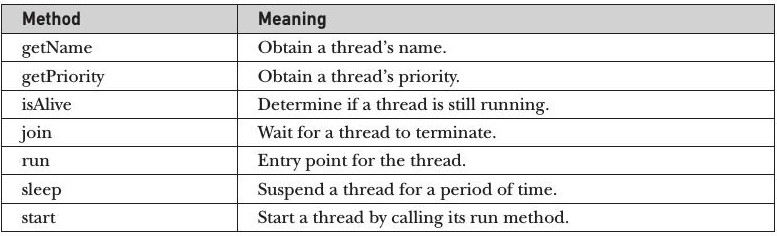
\includegraphics[scale=0.5]{Figures/threadMethods}
\decoRule
\caption{Thread class methods}
\label{fig:threadMethods}
\end{figure}

\subsection{The Main Thread}

A thread begins running when a Java program starts, and it is usually called the main thread. It is used to spawn other child threads and it is the last thread finishing execution and performs some shutdown actions.

\subsection{Creating a thread}

\subparagraph{Implementing Runnable}
To implement Runnable, a class needs to implement only the \textbf{run()} method. Inside this method you define the code that constitues the new thread. The thread will end when run() returns. You have to instantiate a Thread object from within the class that implements Runnable.

\begin{lstlisting}
class NewThread implements Runnable {
  Thread t;

  NewThread() {
    // Create a new, second thread
    t = new Thread(this, "Demo Thread");
    System.out.println("Child thread: " + t);
    t.start(); // Start the thread
  }

  // This is the entry point for the second thread.
  public void run() {
    try {
      for(int i = 5; i > 0; i--) {
        System.out.println("Child Thread: " + i);
        Thread.sleep(500);
      }
    } catch (InterruptedException e) {
      System.out.println("Child interrupted.");
    }
    System.out.println("Exiting child thread.");
  }
}
\end{lstlisting}

\subparagraph{Extending Thread}
Another way to create a thread is to create a class that extends Thread and instantiate it. The entry point of the new thread is the \textbf{run()} method, which has to be overridden. To begin execution of the thread, the new class has to call the start() method.

\begin{lstlisting}
class NewThread extends Thread {

  NewThread() {
    // Create a new, second thread
    super("Demo Thread");
    System.out.println("Child thread: " + this);
    start(); // Start the thread
  }

  // This is the entry point for the second thread.
  public void run() {
    try {
      for(int i = 5; i > 0; i--) {
        System.out.println("Child Thread: " + i);
        Thread.sleep(500);
      }
    } catch (InterruptedException e) {
      System.out.println("Child interrupted.");
    }
    System.out.println("Exiting child thread.");
  }
}
\end{lstlisting}

\subparagraph{isAlive() and join()}

You will often want the main thread to finish last. This can be accomplished by calling sleep(), but the most useful methods are isAlive(), whic returns true if the thread is still alive, or false otherwise, and join(), which waits until the thread on which is called terminates.

\begin{lstlisting}
NewThread ob1 = new NewThread("One");
NewThread ob2 = new NewThread("Two");
NewThread ob3 = new NewThread("Three");
ob1.t.join();
ob2.t.join();
ob3.t.join();
\end{lstlisting}

\subsection{Thread priorities}

The thread scheduler uses thread priorities to decide when a thread should be allowed to run. To set the priority of a thread, we can use the \textbf{setPriority()} method from the Thread class. The values must be in the range \verb|MIN_PRIORITY and MAX_PRIORITY|, currently these values being 1 and 10. The current priority of a thread can be obtained using the \textbf{getPriority()} method.

\section{Syncronization}

\subsection{Using syncronized Methods}

The easiest syncronization method in Java is to use the monitor associated by each object. To enter this monitor, you have to call all method associated with the \textbf{synchronized} keyword. All the other threads that want to call the syncronized method while other thread is inside it have to wait for it to finish.

\subsection{Using syncronized Statement}

To access an object of a class that does not use syncronized methods, you just have to put the calls to that methods inside a syncronized block. The general form of a syncronized block is:
\begin{lstlisting}
syncronized(objRef) {
	//statements to be syncronized
}
\end{lstlisting}

\subsection{Using Syncronization Objects}

To enable handling of several difficult syncronization situations easily, the following syncronization objects are supported: \textbf{Semaphore, CountDownLatch, CyclicBarrier, Exchanger and Phaser}. All these classes are located in the java.util.concurrent package, which defines some core features to support advanced syncronization and interthread communication methods.

\subparagraph{Semaphore}
\subparagraph{CountDownLatch}
\subparagraph{CyclicBarrier}
\subparagraph{Exchanger}
\subparagraph{Phaser}

\section{Using an Executor}

\section{Parallel Programming via the Fork/Join Framework}
% Chapter Template

\chapter{Java 8: Streams and Lambda expressions} % Main chapter title

\label{Chapter2} % Change X to a consecutive number; for referencing this chapter elsewhere, use \ref{ChapterX}

Streams and lamba expressions are the most important new features introduced in Java 8 version. Stream has been added as a method in the Collection interface and other data sources. They allow processing the elements of a data structure to generate new structures and filter the data. They can be used to implement algorithms using the map and reduce technique.

Parallel streams are a special kind of streams which operates in a parallel way. The elements involved in the use of parallel streams are:
\begin{itemize}
\item The Stream interface: defines the operations that can be performed on a stream.
\item Optional: a container object
\item Collectors: implements the reduction operations that are used in a stream sequence of operations.
\item Lambda expressions: most stream methods accept a lambda expression as a parameter, allow more compact operations implementaions.
\end{itemize}

\section{Lambda Expression}

A lambda expression can be understood as a concise representation of an anonymous function that can be passed around: it doesn’t have a name, but it has a list of parameters, a body, a return type, and also possibly a list of exceptions that can be thrown.

\begin{itemize}
\item Anonymous - it doesn’t have an explicit name like a method would normally have.
\item Function - a lambda isn’t associated with a particular class like a method is. But like a method, a lambda has a list of parameters, a body, a return type, and a possible list of exceptions that can be thrown.
\item Passed around - a lambda expression can be passed as argument to a method or stored in a variable.
\item Concise - you don’t need to write a lot of boilerplate like you do for anonymous classes.
\end{itemize}

Lambdas technically don’t let you do anything that you couldn’t do prior to Java 8. But you no longer have to write clumsy code using anonymous classes to benefit from behavior parameterization. The net result is that your code will be clearer and more flexible. For example, using a lambda expression you can create a custom Comparator object in a more concise way:

Without lambda expression:

\begin{lstlisting}
Comparator<Apple> byWeight = new Comparator<Apple>() {
    public int compare(Apple a1, Apple a2){
        return a1.getWeight().compareTo(a2.getWeight());
    }
};
\end{lstlisting}

With lambda expression:
\begin{lstlisting}
Comparator<Apple> byWeight =
    (Apple a1, Apple a2) -> a1.getWeight().compareTo(a2.getWeight());
\end{lstlisting}

\subsection{Where and how to use lambdas}

\paragraph{Functional interface} You can use a lambda expression in the context of a functional interface. A functional interface is an interface that specifies exactly one abstract method. You already know several other functional interfaces in the Java API such as Comparator and Runnable. Interfaces can now also have default methods (that is, a method with a body that provides some default implementation for a method in case it isn’t implemented by a class). An interface is still a functional interface if it has many default methods as long as it specifies only one abstract method. Lambda expressions let you provide the implementation of the abstract method of a functional interface directly inline and treat the whole expression as an instance of a functional interface (more technically speaking, an instance of a concrete implementation of the functional interface). You can achieve the same thing with an anonymous inner class, although it’s clumsier: you provide an implementation and instantiate it directly inline.

\paragraph{Function descriptor} The signature of the abstract method of the functional interface essentially describes the signature of the lambda expression. We call this abstract method a function descriptor. For example, the Runnable interface can be viewed as the signature of a function that accepts nothing and returns nothing (void) because it has only one abstract method called run, which accepts nothing and returns nothing (void). \cite{urma2014java}

\section{Parallel streams}

Stream interface allows you to process its elements in parallel in a very convenient way: it’s possible to turn a collection into a parallel stream by invoking the method parallelStream on the collection source. A parallel stream is a stream that splits its elements into multiple chunks, processing each chunk with a different thread. Thus, you can automatically partition the workload of a given operation on all the cores of your multicore processor and keep all of them equally busy.

Let’s suppose you need to write a method accepting a number n as argument and returning the sum of all the numbers from 1 to the given argument. A straightforward approach is to generate an infinite stream of numbers, limiting it to the passed number, and then reduce the resulting stream with a BinaryOperator that just sums two numbers, as follows:

\begin{lstlisting}
public static long sequentialSum(long n) {
	return Stream.iterate(1L, i -> i + 1)
				  .limit(n)
				  .reduce(0L, Long::sum);
}	
\end{lstlisting}

In more traditional Java terms, this code is equivalent to its iterative counterpart:

\begin{lstlisting}
public static long iterativeSum(long n) {
    long result = 0;
    for (long i = 1L; i <= n; i++) {
        result += i;
    }
    return result;
}	
\end{lstlisting}

This operation seems to be a good candidate to leverage parallelization, especially for large values of n.

You can make the former functional reduction process (that is, summing) run in parallel by turning the stream into a parallel one; call the method parallel on the sequential stream:

\begin{lstlisting}
public static long parallelSum(long n) {
	return Stream.iterate(1L, i -> i + 1)
				  .limit(n)
				  .parallel()
				  .reduce(0L, Long::sum);
}	
\end{lstlisting}
 

%----------------------------------------------------------------------------------------
%	BIBLIOGRAPHY
%----------------------------------------------------------------------------------------
\begingroup
\let\cleardoublepage\clearpage
\printbibliography[heading=bibintoc]
\endgroup
%----------------------------------------------------------------------------------------

\end{document}  
